\documentclass{article}
\usepackage{a4wide}
\usepackage{listings}
\usepackage{graphicx}

\linespread{1.3}

\title{Earth Daemon Plugins}

\begin{document}

\begin{titlepage}
    \begin{center}
        Rising Sun Pictures \\
        \vspace{1cm}
        \begin{center}                
        
\includegraphics{earth.png} \\
        \end{center}
        \vspace{5cm}
        {\LARGE\bf Daemon Plugins} \\
        \vspace{5cm}
        {\LARGE\bf Development Documentation} \\
        \vspace{6cm}
        \today
    \end{center}
\end{titlepage}

\tableofcontents
\listoffigures

\newpage

\section{Introduction} % (fold)
\label{sec:introduction}

\noindent
The plugin concept that is already included as part of the existing Earth Daemon (earthd) design provides a clear indication that extensibility and maintainability are a priority consideration of the Earth application. Within the daemon, the design logic of the file monitor had been removed and implemented as a separate module in a pluggable form. However, the actual implementation had been constructed in such a way that the invocation of the file monitor module can switch between the plugin option or the more direct file inclusion option. This switch is simply activated with the setting or clearing of the LOAD\_FILE\_MONITOR\_AS\_PLUGIN flag. Further investigation revealed that the purpose for retaining this option was to enable the quick alteration and testing of the file monitor module should a necessary modification or update become necessary. With the plugin option, the additional preparatory tasks of signing and installing the plugin is time-consuming and can become intolerable particularly for simple code alterations. \\ 

\noindent
The following sections will present the exploration conducted on the plugins framework, and the modification performed. Also, a quick guide to create and install a plugin. \\

% section introduction (end)

\section{Exploration} % (fold)
\label{sec:exploration}

An exploration on getting a better understanding of the plugin framework was done. It was found that each plugin is a sub-class of the \texttt{EarthPlugin} class. This was discovered while re-reading the \texttt{file\_monitor.rb} file. Figure \ref{fig:plugin} shows the basic structure of an Earth plugin. The codes shown in the mentioned figure are compulsory methods as the File Monitor uses them to retrieve information about the plugin. These compulsory methods will be revisited in later sections. 

\begin{figure}[ht]
    \centering
    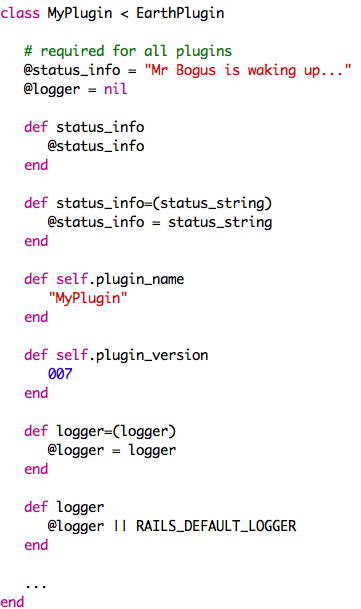
\includegraphics[scale=0.5]{plugin_standard_codes.png}
    \caption{Plugin standard code structure.}
    \label{fig:plugin}
\end{figure}

A further exploration was done to understand how a plugin is invoked from the daemon. It was found that each plugin is stored and retrieved from the database. The table that stores the plugins is the \texttt{plugins\_descriptors} table. The following is the table's schema:

\begin{verbatim}
    create_table "plugin_descriptors", :force => true do |t|
    t.string  "name",           :limit => 64, :null => false
    t.integer "version",                      :null => false
    t.binary  "code",                         :null => false
    t.binary  "sha1_signature",               :null => false
  end

  add_index "plugin_descriptors", ["name"], :name => "plugin_descriptors_unique_name", 
                                            :unique => true
\end{verbatim}

This table will be revisited in later sections as well as further investigation found that the \texttt{code} and \texttt{sha1\_signature} columns are not compatible with the PostgresSQL RubyGem connector. Figure \ref{fig:flow} shows the flow of plugins being loaded in Earth.

\begin{figure}[ht]
    \centering        
    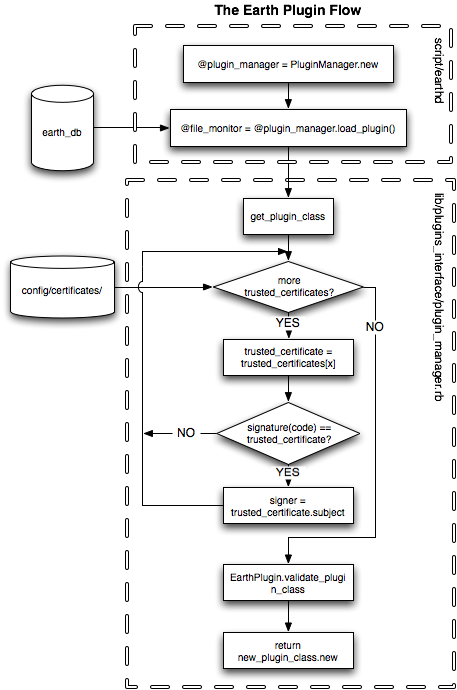
\includegraphics[scale=0.5]{flow.png}
    \caption{Plugin loading flow.}
    \label{fig:flow}
\end{figure}

It is now understood that the reason why the plugins are stored and loaded from database, instead of loading them from individual files. This is because each daemon is executed in different machines on the network, and the daemons relay files and directories information between the main database server and the file servers that they are monitoring. Thus, for a quick and clean plugin loading, the best solution is to have them loaded remotely and dynamically from a database, provided the plugin is not too complex. 

% section exploration (end)

\section{Security Retrofitting} % (fold)
\label{sec:security_retrofitting}

From the Figure \ref{fig:flow}, it is understood that plugins are to be dynamically and remotely loaded from the database, and there is a security processing overhead imposed on the load time. This is a mandatory overhead imposed as remote plugin calls can be susceptible to `man in the middle attack', which a hacker can modify the codes during transmission for any malicious act. The challenge now is to have File Monitor loaded into the database. However, it was found that the \texttt{sign\_plugin} and \texttt{create\_cert} scripts were not updated to be compatible with Rails 2.0.2. The following codes were updated to \texttt{require\_gem `termios'}: 

\begin{verbatim}
    gem 'termios'
    require 'termios'
\end{verbatim}

The listed codes are the new syntax statements used to include the \texttt{termios} gem. After the certifications, signing and installation, it was later found that the plugin do not load properly when the flag was set to \texttt{true}. Further investigation was performed, and it was found that the both the \texttt{code} and \texttt{sha1\_signature} columns have been `flatten' to UTF codes, instead of the original characters used. Thus causing the verification to fail. It was also found that even without the verification, the plugin failed to load. As such, a mitigation action was performed to have this problem fixed. It was speculated that perhaps it is this problem that the flag was turned off. This is a known problem between PostgresSQL and Ruby, where the data being transferred are `lost in translation' between UTF and plaintext when the data are stored in \texttt{binary} type. The following is the fix towards this problem:

\begin{verbatim}
    class ChangePluginDescriptorCodeSignatureColumnsToText < ActiveRecord::Migration
      def self.up
        change_column :plugin_descriptors, :code, :text
        change_column :plugin_descriptors, :sha1_signature, :text
      end

      def self.down
        change_column :plugin_descriptors, :code, :binary
        change_column :plugin_descriptors, :sha1_signature, :binary
      end
    end
\end{verbatim}

This is the first step towards fixing the problem, which is to have the \texttt{binary} columns updated to \texttt{text} columns. The second step is to encode the codes and signatures using a reversible encoding, which plaintext is used as the encoded text. The solution is to use the Base64 encoding class that is bundled with Ruby. The following changes were added into the \texttt{plugin\_manager.rb} file, which is the plugin management class:

\begin{verbatim}
    # To load it into the database
    b64_code = Base64.b64encode(code)
    b64_signature = Base64.b64encode(signature)
    
    # To load from the database
    code = Base64.decode64(newPlugin.code)
    signature = Base64.decode64(newPlugin.sha1_signature)
\end{verbatim}

This will allow the code and signature to be stored and loaded from the database without loosing integrity. 

% section security_retrofitting (end)

\section{Plugin Framework Re-implementation} % (fold)
\label{sec:plugin_framework_re-implementation}

After the first rounds of retrofitting, another challenge arise, which is to allow a plugin to be plug-able as well. In the other words to have Earth support plugins of plugins. In the beginning, the idea of re-writing Earth to introduce an Application Programmable Interface (API) was used. However, this idea was gradually dropped due to the very monolithic design. Thus, a new idea was explored, which is to include extensions into the plugins. Figure \ref{fig:framework} shows the re-implemented plugin framework, from the \texttt{earthd}'s point of view. 

\begin{figure}[ht]
    \centering
    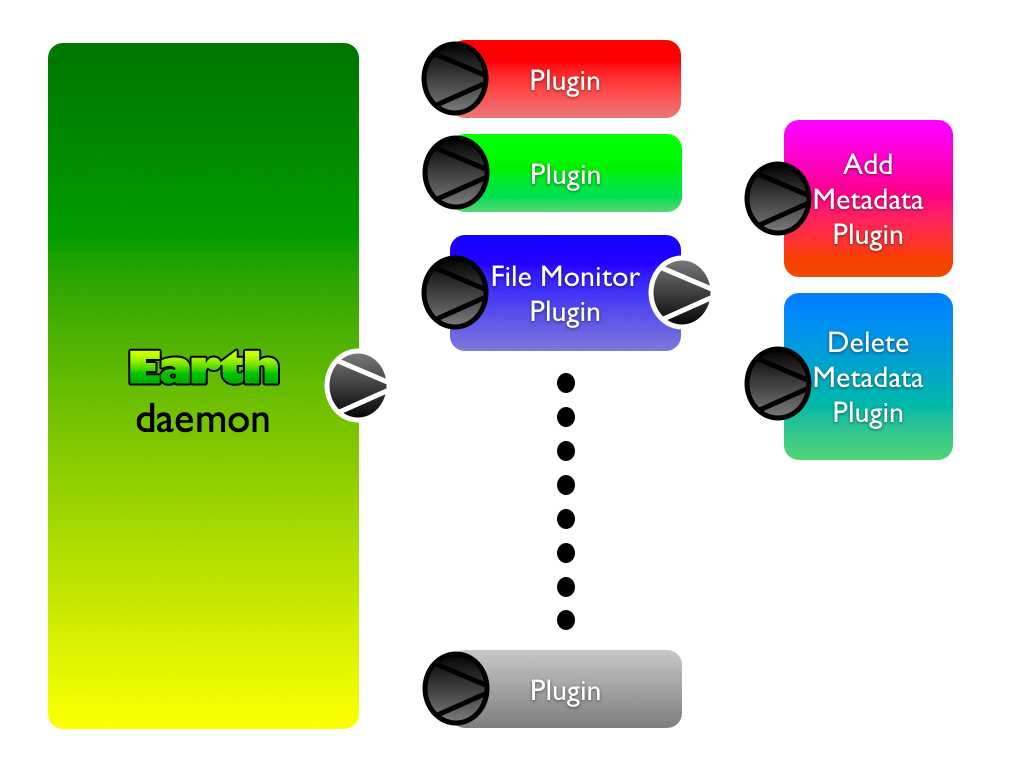
\includegraphics[scale=0.4]{daemon_plugins.png}
    \caption{The re-implemented plugin framework.}
    \label{fig:framework}
\end{figure}

The current plugin framework do not support such a framework. Thus, a new extension module was developed, which is included when the daemon is launched. The following line can be added into the plugin intended for extension:

\begin{verbatim}
    extension_point(<the extension point name>, <class name>, <list of variables>)
\end{verbatim}

% section plugin_framework_re-implementation (end)

\section{Plugin Creation} % (fold)
\label{sec:plugin_creation}

To create a plugin, all one needed to do is to follow the coding scheme as shown in Figure \ref{fig:plugin}. To illustrate how can this be done, the following is a sample code of a blank plugin called Mr Bogus:

\begin{verbatim}
    class BogusPlugin < EarthPlugin
      def self.plugin_name
        "EarthBogusPlugin"
      end

      def self.plugin_version
        1
      end

      def initialize
        #bring the parameters from the plug-in session
        @logger = get_param(:logger)
        @logger.debug("Mr Bogus... he is the hero!!");
      end
    end    
\end{verbatim}

This plugin will be loaded by the daemon and prints out \texttt{Mr Bogus... he is the hero!!} in the log file, which can be found in the \texttt{temp/earthd.log} file. As compared to the original listing in Figure \ref{fig:plugin}, some of the methods were dropped as this plugin is too simple to have those methods. However, the listed methods above is important and must not be dropped. 

% section plugin_creation (end)

\section{Installation} % (fold)
\label{sec:installation}

The following are the steps to have a plugin installed:

\begin{enumerate}
    \item Run \texttt{script/create\_cert} to generate a certificate of the host system. (One will need to create directories \texttt{config/certificates} and \texttt{config/keys} in order this script to work. 
    \item Run \texttt{script/earth\_plugins sign <plugin\_file>} to create a \texttt{*.sha1} signature file. 
    \item (Optional) Run \texttt{script/console} to check whether the signature is valid. (NOTE: At this stage, one should have created 3 files: \texttt{config/certificates/test\_cert.pem}, \texttt{config/keys/test\_key.pem} and \texttt{<plugin>.rb.sha1})
        \begin{enumerate}
            \item Run \texttt{signature = File.read(``<plugin>.rb.sha1'')}
            \item Run \texttt{code = File.read(``<plugin>.rb'')}
            \item Run \texttt{cert = OpenSSL::X509::Certificate.new( \\ File::read(``config/certificates/test\_cert.pem''))}
            \item Run \texttt{cert.public\_key.verify(OpenSSL::Digest::SHA1.new, signature, code)}. (One should get \texttt{true} as the result after running this line.)
        \end{enumerate}
    \item Run \texttt{script/earth\_plugins install <plugin\_file> <extension\_point> <attached\_plugin>} to install. The extension point is \textbf{\texttt{main\_loop}} if the plugin is attached to the daemon, which is \textbf{\texttt{Earthd}}. 
\end{enumerate}

At this stage, the plugin should be installed, and the \texttt{earth\_plugins} script will print out all the Base64 encoding on screen without any error. To verify the plugin is indeed installed, one can invoke the following command, which will list all the installed plugins in the database:

\begin{verbatim}
    script/earth_plugins list info
\end{verbatim}

% section installation (end)

\section{Uninstallation} % (fold)
\label{sec:uninstallation}

To uninstall a plugin, the following command can be used:

\begin{verbatim}
    script/earth_plugins uninstall <plugin_name>
\end{verbatim}

One can obtain the plugin name from the list command, as stated in the previous section.

% section uninstallation (end)

\end{document}  